\documentclass[a4paper]{article}

\usepackage{polyglossia}
\setdefaultlanguage{russian}
\usepackage{fontspec}
\setmainfont{Times New Roman}
\newfontfamily\cyrillicfont{Times New Roman}
\newfontfamily\cyrillicfonttt{FreeMono}

\usepackage{graphicx}
\usepackage{float}
\usepackage{wrapfig}
\usepackage{tikz}
\usepackage{svg}

\usepackage{amsmath, amssymb}

\usepackage{hyperref}
\definecolor{urlcolor}{rgb}{0,0,1}
\definecolor{linkcolor}{rgb}{0,0,0.8}
\hypersetup{
  pdfborder=0 0 0,
  pdfstartview=FitH,
  linkcolor=linkcolor,
  urlcolor=urlcolor,
  colorlinks=true
}

\usepackage{caption}
\usepackage{geometry}
\geometry{left=2cm, right=2cm, top=2cm, bottom=2cm}

\usepackage{fancyhdr}
\usepackage{nicefrac}

\usepackage{xcolor}
\definecolor{strings}{rgb}{0,0.6,0}
\definecolor{comments}{rgb}{0,0.3,0}
\definecolor{numbers}{rgb}{0.5,0.5,0.5}
\definecolor{keywords}{rgb}{0.09,0.61,0.95}
\definecolor{background}{rgb}{0.97,0.97,0.97}

\usepackage{listings}

\lstdefinestyle{codestyle}{
    backgroundcolor=\color{background},
    commentstyle=\color{comments},
    keywordstyle=\color{keywords},
    stringstyle=\color{strings},
    numberstyle=\tiny\color{numbers},
    basicstyle=\ttfamily\footnotesize,
    breakatwhitespace=false,
    breaklines=true,
    captionpos=b,
    inputencoding=utf8,
    keepspaces=true,
    numbers=left,
    numbersep=5pt,
    showspaces=false,
    showstringspaces=false,
    showtabs=false,
    tabsize=2,
    extendedchars=true,
    literate=
      {а}{{\cyra}}1 {б}{{\cyrb}}1 {в}{{\cyrv}}1 {г}{{\cyrg}}1
      {д}{{\cyrd}}1 {е}{{\cyre}}1 {ж}{{\cyrzh}}1 {з}{{\cyrz}}1
      {и}{{\cyri}}1 {й}{{\cyrishrt}}1 {к}{{\cyrk}}1 {л}{{\cyrl}}1
      {м}{{\cyrm}}1 {н}{{\cyrn}}1 {о}{{\cyro}}1 {п}{{\cyrp}}1
      {р}{{\cyrr}}1 {с}{{\cyrs}}1 {т}{{\cyrt}}1 {у}{{\cyru}}1
      {ф}{{\cyrf}}1 {х}{{\cyrh}}1 {ц}{{\cyrc}}1 {ч}{{\cyrch}}1
      {ш}{{\cyrsh}}1 {щ}{{\cyrshch}}1 {ъ}{{\cyrhrdsn}}1 {ы}{{\cyrery}}1
      {ь}{{\cyrsftsn}}1 {э}{{\cyrerev}}1 {ю}{{\cyryu}}1 {я}{{\cyrya}}1
      {А}{{\CYRA}}1 {Б}{{\CYRB}}1 {В}{{\CYRV}}1 {Г}{{\CYRG}}1
      {Д}{{\CYR96}}1 {Е}{{\CYRE}}1 {Ж}{{\CYRZH}}1 {З}{{\CYRZ}}1
      {И}{{\CYRI}}1 {Й}{{\CYRISHRT}}1 {К}{{\CYRK}}1 {Л}{{\CYRL}}1
      {М}{{\CYRM}}1 {Н}{{\CYRN}}1 {О}{{\CYRO}}1 {П}{{\CYRP}}1
      {Р}{{\CYRR}}1 {С}{{\CYRS}}1 {Т}{{\CYRT}}1 {У}{{\CYRU}}1
      {Ф}{{\CYRF}}1 {Х}{{\CYRH}}1 {Ц}{{\CYRC}}1 {Ч}{{\CYRCH}}1
      {Ш}{{\CYRSH}}1 {Щ}{{\CYRSHCH}}1 {Ъ}{{\CYRHRDSN}}1 {Ы}{{\CYRERY}}1
      {Ь}{{\CYRSFTSN}}1 {Э}{{\CYREREV}}1 {Ю}{{\CYRYU}}1 {Я}{{\CYRYA}}1
}

\lstset{style=codestyle}

\begin{document}

\begin{titlepage}
    \centering
    {\large Федеральное государственное автономное образовательное учреждение\par}
    {\large высшего образования\par}
    {\bfseries САНКТ-ПЕТЕРБУРГСКИЙ НАЦИОНАЛЬНЫЙ ИССЛЕДОВАТЕЛЬСКИЙ УНИВЕРСИТЕТ ИТМО\par}
    \vfill
    {\Large \bfseries Исследовательский проект \par}
    {\Large Факторы, влияющие на размер среднего чека и вероятность повторной покупки в интернет-магазине \par}
    \vfill
    
    \begin{flushright}
        Студенты: \\
            Большакова Я.Н. МатСтат 22.5 \\
            Гизбрехт В.Д. МатСтат 22.5 \\
            Кашапова А.К. МатСтат 22.5 \\
            Сайфуллин Д.Р. МатСтат 22.5 \\
            Солдатова А.А. МатСтат 22.4 \\
        Преподаватель: \\
            Яворук Т.О.\\
    \end{flushright}
    \vfill
    Санкт-Петербург \\
    2025 г.
\end{titlepage}

\tableofcontents
\newpage

\section{Постановка задачи}
В условиях быстрорастущего рынка электронной коммерции понимание факторов, формирующих поведение покупателей, является ключевым для повышения эффективности маркетинга и оптимизации бизнес-процессов. Одним из важных показателей, отражающих ценность клиента, является средний чек (Average Order Value, AOV), в то время как вероятность повторной покупки служит индикатором лояльности и потенциального пожизненного дохода клиента.


\subsection*{Цели исследования:}
Выявить и количественно оценить факторы, влияющие на:
\begin{itemize}
  \item размер среднего чека (AOV);
  \item вероятность совершения повторной покупки в течение 30 дней.
\end{itemize}


\subsection*{Гипотезы:}
Предварительно сформулированы три основные гипотезы:

\begin{enumerate}
  \item Частота покупок ($\mathrm{freq}$) и суммарная выручка ($\mathrm{mon}$) статистически значимо влияют на размер среднего чека:
    \[
      \mathrm{AOV} = \beta_0 + \beta_1\,\mathrm{freq} + \beta_2\,\mathrm{mon} + \varepsilon.
    \]

  \item Средний чек различается в зависимости от региона (\(\mathrm{region}\)) клиента:
    \[
      \mathrm{AOV}_i \sim \mathcal{N}(\mu_{\mathrm{region}_i}, \sigma^2),
      \quad i=1,\dots,n.
    \]
    Проверка — однофакторный дисперсионный анализ.

  \item Среднее количество товаров в корзине (\(\mathrm{AvgQty}\)) отличается у клиентов, совершивших повторную покупку (\(\mathrm{repeat}=1\)), и у тех, кто не повторил покупку (\(\mathrm{repeat}=0\)):
    \[
      H_0: \mathbb{E}[\mathrm{AvgQty}\mid \mathrm{repeat}=1] = \mathbb{E}[\mathrm{AvgQty}\mid \mathrm{repeat}=0],
    \]
    проверка — двухвыборочный t-тест для независимых выборок.
\end{enumerate}

\section{Теория}

В этом разделе мы коротко разберём основные методы, которые будем применять.

\subsection{RFM и средний чек}
RFM-анализ помогает поймать самые важные характеристики покупателя:
\begin{itemize}
  \item \textbf{Recency} — как давно была последняя покупка;
  \item \textbf{Frequency} — сколько раз купил клиент;
  \item \textbf{Monetary} — сколько всего потратил.
\end{itemize}
Из этого легко получить средний чек:
\[
  \text{AOV} = \frac{\text{Monetary}}{\text{Frequency}}.
\]

\subsection{Линейная регрессия}
Чтобы проверить, как частота и выручка связаны с AOV, используем простую линейную модель:
\[
  \text{AOV} = \beta_0 + \beta_1\,\text{freq} + \beta_2\,\text{mon} + \varepsilon.
\]
Метод наименьших квадратов подбирает коэффициенты так, чтобы минимизировать сумму квадратов ошибок.

\subsection{Дисперсионный анализ (ANOVA)}
ANOVA помогает сравнить средние нескольких групп. Если у нас есть разные регионы, мы смотрим, насколько сильно отличаются их средние AOV.  
Статистика \(F\) показывает отношение «межгрупповой» вариативности к «внутригрупповой». Малое \(p\)-значение говорит, что средние действительно разные.

\subsection{t-тест для двух групп}
Чтобы убедиться, что у тех, кто вернулся за покупкой, среднее количество товаров в корзине (AvgQty) отличается от тех, кто не вернулся, делаем t-тест:
\[
  t = \frac{\bar x_1 - \bar x_0}{\sqrt{\frac{s_1^2}{n_1} + \frac{s_0^2}{n_0}}},
\]
где \(\bar x\) и \(s^2\) — средние и дисперсии в группах, \(n\) — размер выборки.  

Если \(p<0.05\), значит разница средних значимая.

\section{Использованные программные средства}

Для обработки данных и выполнения всех вычислений мы использовали следующий инструментарий:

\begin{itemize}
  \item \textbf{Язык программирования:} Python 3.9
  \item \textbf{Основные библиотеки:}
    \begin{itemize}
      \item \texttt{pandas} для чтения CSV и агрегации данных
      \item \texttt{scipy.stats} для статистических тестов (корреляция, ANOVA, t-тест)
      \item \texttt{statsmodels} для линейной и логистической регрессии
    \end{itemize}
  \item \textbf{Среда разработки:}
    \begin{itemize}
      \item Visual Studio Code для написания и отладки кода
    \end{itemize}
  \item \textbf{Система контроля версий:} Git, репозиторий с кодом доступен по ссылке:\\
    \url{https://github.com/yourusername/ecommerce-rfm-analysis}
  \item \textbf{Дополнительные ресурсы:}
    \begin{itemize}
      \item The Complete Journey: \url{https://www.dunnhumby.com/source-files/}
      \item Руководство по Dunnhumby “The Complete Journey” (см. User Guide PDF)
    \end{itemize}
\end{itemize}

\section{Результаты}

Ниже приведены ключевые статистики и графики по каждой из проверенных гипотез.

\subsection{Результаты H1: Частота и выручка → AOV}

\begin{figure}[H]
  \centering
  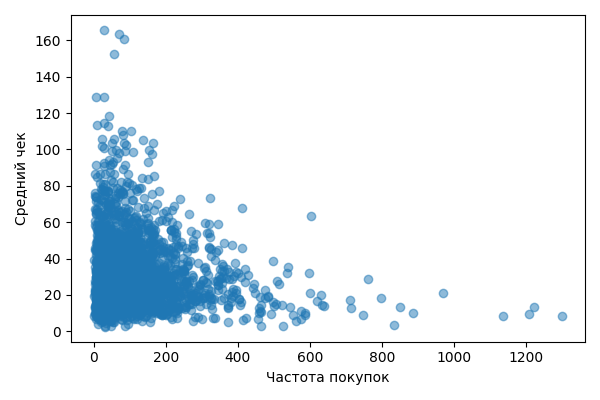
\includegraphics[width=0.45\textwidth]{img/freq_vs_aov.png}
  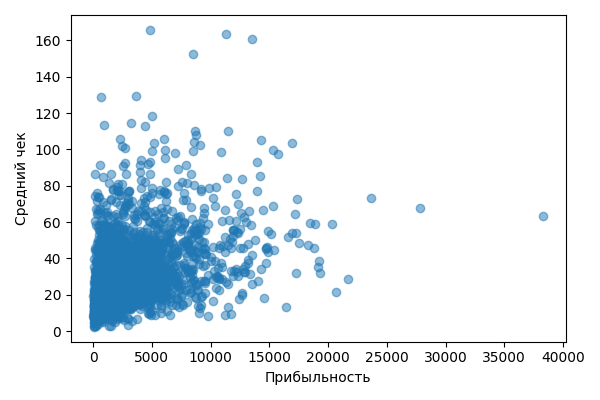
\includegraphics[width=0.45\textwidth]{img/mon_vs_aov.png}
  \caption{Зависимость AOV от Частоты покупок (слева) и от Прибыли (справа).}
  \label{fig:h1_scatter}
\end{figure}

\begin{table}[H]
  \centering
  \begin{tabular}{lrrr}
    Предиктор & Коэффициент & t-статистика & P-значение \\
    \(\mathrm{freq}\) & \(-0.1296\) & \(-38.221\) & \(<0.001\) \\
    \(\mathrm{mon}\)  & \(+0.0054\) & \(+45.772\) & \(<0.001\) \\
  \end{tabular}
  \caption{Коэффициенты регрессии \(\mathrm{AOV} = \beta_0 + \beta_1\,\mathrm{freq} + \beta_2\,\mathrm{mon}\).}
  \label{tab:h1_coef}
\end{table}

\noindent
\textbf{Вывод.} Корреляции \(\rho(\text{freq},\text{AOV})=-0.124\) (\(p\ll0.001\)) и \(\rho(\text{mon},\text{AOV})=+0.389\) (\(p\ll0.001\)) и результаты анализа (см. табл.~\ref{tab:h1_coef}, \(R^2=0.465\)) подтверждают гипотезу H1:  
\begin{itemize}
  \item С увеличением \(\mathrm{mon}\) средний чек растёт.
  \item С увеличением \(\mathrm{freq}\) средний чек слегка снижается.
\end{itemize}

\subsection{Результаты H2: Регион → AOV}

\begin{figure}[H]
  \centering
  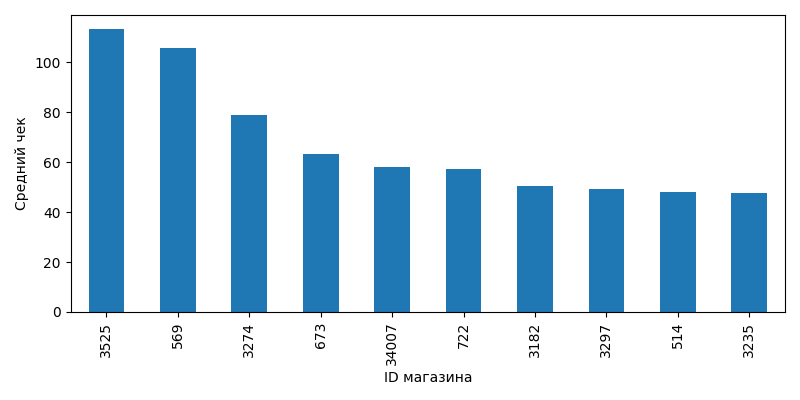
\includegraphics[width=0.7\textwidth]{img/top_stores_mean_aov.png}
  \caption{ТОП-10 магазинов по среднему чеку.}
  \label{fig:top10_stores}
\end{figure}

\begin{table}[H]
  \centering
  \begin{tabular}{lr}
    ID магазина & {Mean AOV} \\
    3525 & 113.32 \\
    569  & 105.95 \\
    3274 &  78.99 \\
    673  &  63.37 \\
    34007&  58.01 \\
    722  &  57.21 \\
    3182 &  50.62 \\
    3297 &  49.48 \\
    514  &  48.10 \\
    3235 &  47.67 \\
  \end{tabular}
  \caption{Средний чек по ТОП-10 магазинам.}
  \label{tab:top10}
\end{table}

\noindent
ANOVA по всем магазинам дала \(F=1.99\), \(p<0.001\), что говорит о статистически значимых различиях средних AOV между магазинами. Рис.~\ref{fig:top10_stores} и табл.~\ref{tab:top10} демонстрируют, что наиболее высокие средние чеки наблюдаются в магазинах 3525 и 569, а наименьшие — в более мелких точках.

\subsection{Результаты H3: Среднее количество товаров в корзине у повторных и неповторных покупателей}

\begin{figure}[H]
  \centering
  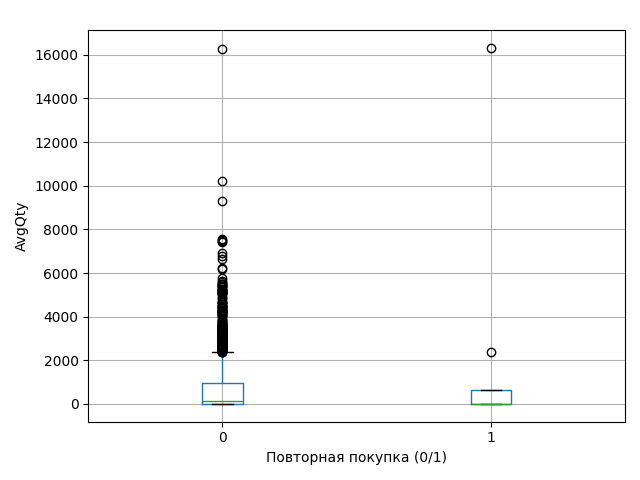
\includegraphics[width=0.6\textwidth]{img/boxplot_avgqty_repeat.png}
  \caption{Распределение AvgQty для клиентов с repeat=0 и repeat=1.}
  \label{fig:h3_box}
\end{figure}

\begin{table}[H]
  \centering
  \begin{tabular}{lrr}
    Группа & Среднее AvgQty & n \\
    repeat = 1 & 2349.56 & 8 \\
    repeat = 0 &  721.49 & 2492 \\
  \end{tabular}
  \caption{Среднее количество штук товара в корзине по группам.}
  \label{tab:h3_means}
\end{table}

\noindent
t-тест для H3 дал \(t=0.81\), \(p=0.446\) (табл.~\ref{tab:h3_means}), то есть статистически значимой разницы в AvgQty между повторщиками и однократниками не выявлено. Это может быть связано с тем, что в группе повторщиков всего 8 человек, при этом в обеих группах есть отдельные очень крупные значения AvgQty, что сильно искажает среднее.

Таким образом, гипотезы H1 и H2 подтверждены, а H3 опровергнута при уровне значимости 0.05.

\section{Обсуждение}
В ходе исследования удалось подтвердить две ключевые гипотезы:  
— зависимость среднего чека от суммарной выручки и частоты покупок (H1) показала сильную статистическую значимость и логическую интерпретацию: крупные единовременные траты растят AOV, а частые мелкие покупки, наоборот, его снижают.  
— различие средних чеков между магазинами (H2) также достоверно, что позволяет выделять точки-лидеры и перераспределять маркетинговые усилия.

Гипотеза H3 о том, что у повторных покупателей среднее количество товаров в корзине существенно выше, формально не подтвердилась: узкое окно повторных покупок (30 дней), малое число повторщиков и экстремальные выбросы сделали среднее нечувствительным тестируемым параметром. Это указывает на то, что для анализа повторного поведения необходимо либо расширить окно наблюдения, либо перейти к метрикам, устойчивым к выбросам (медиана, логарифмическое преобразование, непараметрические методы).

\section{Заключение}
В ходе выполнения данной проектной работы нами были приобретены и закреплены практические навыки работы с реальными данными, полученными из открытых источников. Этот опыт оказался чрезвычайно ценным, поскольку позволил не только применить теоретические знания на практике, но и лучше понять специфику работы с эмпирическими данными, их особенности, а также типичные трудности, возникающие при анализе информации, собранной в естественных условиях, вне искусственно созданных моделей или учебных датасетов.

Особое внимание в рамках исследования уделялось использованию методов математической статистики, которые сыграли ключевую роль в обработке и интерпретации полученных данных. Применение таких методов дало возможность формализовать процесс анализа, повысить точность и объективность выводов, а также обеспечить их статистическую обоснованность. В частности, нами были использованы такие подходы, как вычисление основных статистических характеристик (среднее значение, медиана, дисперсия, стандартное отклонение), построение распределений, проверка гипотез, а также корреляционный и регрессионный анализ — всё это способствовало более глубокому пониманию структуры данных и взаимосвязей между переменными.

Таким образом, проведённая работа не только способствовала достижению поставленных целей и проверке выдвинутых гипотез, но и послужила важным этапом в освоении методов анализа реальных данных с применением математико-статистического аппарата. Полученный в ходе исследования опыт имеет не только теоретическую, но и практическую значимость, поскольку может быть использован в дальнейших исследованиях, связанных с анализом поведения пользователей, прогнозированием тенденций и принятием решений на основе данных.
\end{document}